\scanpage{530}
% E530-01
\mspage{568}
\uline{$\overline{\mathrm{IV}}$}\quad
% E530-02
\deleted{Let}

% E530-03
So let $\mathcal{G}$ be a profinite group, equipped \unsure{with the|with}
% E530-04
\inserted{generators}
$\rho,\sigma\in\mathcal{G}$ satisfying the relations
% E530-05
\[
(1)\qquad \rho^6=\sigma^4=1,\qquad
\rho^3=\sigma^2\quad (\overset{\mathrm{dfn}}{=}\text{``$-1$''}) .
\]
% E530-06
\margin{This simply means that we give ourselves a surjective homomorphism
% E530-07
\diagram{\begin{tikzcd}[ampersand replacement=\&]
\mathrm{SL}(2,\mathbb Z)^{\wedge}\arrow[r] \& \mathcal{G}
\end{tikzcd}}}

% E530-08
A particularly interesting case is the one where
$\rho^3=\sigma^2=1$, to which nevertheless \unsure{I} would not
\unsure{wish} to limit myself. Let $\tau$ be an \unsure{automorphism}
of $\mathcal{G}$ satisfying
% E530-09
\[
(2)\qquad
\tau(\deleted{\unsure{\rho}}\inserted{\sigma})=
\begin{array}{c}\sigma^{-1}\\[-2pt]\inserted{=-\sigma}\end{array},
\qquad \tau(\rho)=\sigma(\rho^{-1})
\]
% E530-10
\margin{Let us introduce \deleted{\unsure{the}} right away the
\unsure{equivalent} element $\tau'=\sigma^{-1}\tau$ satisfying
$\tau'(\rho)=\rho^{-1}$, $\tau'(\sigma)=\sigma^{-1}$
$(\tau'(\varepsilon_0)=\varepsilon_1^{-1},\tau'(\varepsilon_1)=\varepsilon_0^{-1})$.}
% E530-11
(which means that $\tau_\infty$ ``passes to the quotient'' as an
\unsure{automorphism} $\tau$ of $\mathcal{G}$), which implies
% E530-12
\[
(3)\qquad \tau^2=1
\]
% E530-13
\[
(4)\qquad \tau(\varepsilon_0)=\varepsilon_0^{-1},\qquad
\tau(\varepsilon_1)=\varepsilon_1^{-1},\qquad\text{where}
\]
% E530-14
\[
(5)\qquad
\begin{array}{c}
\varepsilon_0=\deleted{\unsure{\alpha}}\sigma\rho\\[-2pt]
\inserted{=-\sigma^{-1}\rho}
\end{array},\qquad
\varepsilon_1=\rho\sigma=\sigma(\varepsilon_0)
=\sigma^{-1}(\varepsilon_0)=\rho(\varepsilon_0).
\]
% E530-15
\margin{\unsure{of the formula}\ \unsure{forgotten}\ \unsure{a} sign $-$,
whereas \unsure{we could} \unsure{from the outset|ask}
simply \unsure{give|take}
$\varepsilon_0=\unsure{\sigma_\infty|\sigma^{-1}}\rho\ldots$}

% E530-16
Put
% E530-17
\[
(5)\qquad \mathcal{G}'=\{1,\tau\}\mathbin{.}\mathcal{G},
\]
% E530-18
so we have
% E530-19
\[
(6)\qquad
\diagram{\begin{tikzcd}[ampersand replacement=\&]
1\arrow[r]\&\mathcal{G}\arrow[r]\&\mathcal{G}'\arrow[r]\&
\{1,\tau\}\arrow[r]\&1.
\end{tikzcd}}
\]

% E530-20
Let
% E530-21
\deleted{\unsure{(7)}}
% E530-22
\[
\begin{gathered}
B_{\rho,\sigma}\subset\operatorname{Aut}(\mathcal{G})\times\widehat{\mathbb Z}^{*}
\\
(7)\qquad =\left\{(u,\mu)\ \left|\
\begin{array}{l}
u(\varepsilon_0)=\varepsilon_0^\mu\\
\deleted{\text{and}}\ u(\sigma)\ \text{conjugate in }\mathcal{G}\text{ to }\sigma^\mu\\
u(\rho)\quad\rule{4cm}{0.3pt}\quad
\mathcal{G}^{\deleted{\unsure{\prime}}}\text{ to }\rho^\mu
\end{array}\right.\right\}.
\end{gathered}
\]
% E530-23
which is obviously a \uline{subgroup}.
The third condition \unsure{can be made explicit} moreover,
% E530-24
\margin{529}

% E530-F01
\margin{\begin{center}
529\\
\texttt{https://grothendieck.umontpellier.fr}\\
Université de Montpellier, UMR CNRS 5149, Case courrier 051, Place Eugène Bataillon\\
34095 Montpellier cedex 5 - France
\end{center}}

\scanpage{531}
% E531-01
since $\rho^6=1$ i.e. $\rho^\mu$ depends only on the image
of $\mu$ in
% E531-02
\[
(\mathbb Z/6\mathbb Z)^*\simeq
\inserted{(\mathbb Z/2\mathbb Z)^*\times}
(\mathbb Z/3\mathbb Z)^*\simeq(\mathbb Z/3\mathbb Z)^*\simeq\pm1,
\]
% E531-03
\deleted{\unsure{only} on \illegible{1}}
% E531-04
\inserted{so}
% E531-05
\[
(8)\qquad \rho^\mu=\rho^{\varepsilon_3(\mu)}
\]
% E531-06
that for $\varepsilon_3(\mu)=1$
% E531-07
\deleted{we}
$u(\rho)$ is conjugate to $\rho$ in $\mathcal{G}$, and for
$\varepsilon_3(\mu)=-1$ it is conjugate to $\rho^{-1}$ in
$\mathcal{G}$, or again to $\rho$ by an element of
$\mathcal{G}'$ -- i.e. an element of the form $\alpha_1\tau_\infty$
with $\alpha_1\in\mathcal{G}$ (since
$\tau_\infty(\rho)=\inserted{\sigma}(\rho^{-1})$ precisely\ldots).
% E531-08
\deleted{We shall thus have,}
% E531-09
\deleted{\[
(9)\qquad u(\rho)=\zeta\rho,\qquad u(\sigma)=\eta\sigma
\quad(\zeta,\eta\in\mathcal{G})
\]}
% E531-10
\deleted{relations}
% E531-11
\deleted{\[
(10)\qquad \zeta=\alpha\rho(\alpha)^{-1},
\qquad\eta=\beta
\]}
% E531-12
We see likewise that we have
% E531-13
\[
\begin{aligned}
(9)\qquad \sigma^\mu=\sigma^{\varepsilon_2(\mu)}
&\quad\left\{\begin{array}{ll}
=\sigma&\text{if }\mu\equiv1\quad(4)\\
\deleted{\unsure{=}}\sigma^{-1}=-\sigma
&\text{if }\mu\equiv-1\quad(4)
\end{array}\right.\\[-2pt]
&\hspace{2.5cm}\deleted{=\unsure{\varepsilon\sigma|\sigma}}\\
&=\varepsilon_2(\mu)\sigma
\end{aligned}
\]
% E531-14
\deleted{But So \unsure{even|=} \unsure{we write}
(for $(u,\mu)\in B_{\rho,\sigma}$) some
\deleted{\unsure{such $\alpha\in$}} elements
$\alpha\in\mathcal{G}'$, $\beta\in$}

% E531-15
Thus:

% E531-16
\uline{Proposition}\quad For \unsure{a|one}
% E531-17
\deleted{have}
$(u,\mu)\in\operatorname{Aut}
(\deleted{\unsure{B_{\rho,\sigma}}}\inserted{\mathcal{G}})
\times\widehat{\mathbb Z}^{*}$ to be in $B_{\rho,\sigma}$,
it is necessary and sufficient that there exist
$\alpha\in\mathcal{G}'_{\deleted{\unsure{\rho,\sigma}}}
{}^{\deleted{\unsure{\varepsilon_3}}}$,
$\beta\in\mathcal{G}$ such that we have
% E531-18
\margin{530}

% E531-F01
\margin{\begin{center}
530\\
\texttt{https://grothendieck.umontpellier.fr}\\
Université de Montpellier, UMR CNRS 5149, Case courrier 051, Place Eugène Bataillon\\
34095 Montpellier cedex 5 - France
\end{center}}

\scanpage{532}
% E532-01
\mspage{569}
% E532-02
\[
(10)\qquad \unsure{u}(\rho)=\operatorname{int}(\alpha)(\rho),\qquad
u(\sigma)=\underbrace{\varepsilon_2(\mu)}_{\varepsilon}
\operatorname{int}(\beta)(\sigma)
\]
% E532-03
and finally
% E532-04
\[
(11)\qquad u(\varepsilon_0)=\varepsilon_0^\mu,
\]
% E532-05
where in addition we have
% E532-06
\deleted{\[
(12)\qquad
\alpha\overset{\inserted{\in\mathcal{G}}}{\unsure{\bmod}\mathcal{G}}
\equiv\tau^{\overset{\inserted{\unsure{\nu_3}}}
{\unsure{\varepsilon_3(\mu)}}}
\quad\overset{\inserted{\mu\equiv1\ (3)}}{(\mathcal{G})}
\quad\text{i.e. }\alpha\in\mathcal{G}\unsure{\Longleftrightarrow}\mu.
\]}
% E532-07
\margin{i.e. $\unsure{\alpha}\equiv\tau$.}

% E532-08
We shall note that
% E532-09
\deleted{$u$}\inserted{$(u,\mu)$}
is uniquely determined by
% E532-10
\inserted{$\mu$ and}
the knowledge of $\alpha$
% E532-11
\inserted{and}
of $\beta$,
% E532-12
\deleted{and of $\varepsilon_2(\mu)$}
and even \unsure{only} by $\mu$ and
% E532-13
\[
(13)\qquad \zeta=\alpha\rho(\alpha)^{-1},\qquad
\eta=\varepsilon_2(\mu)\beta\sigma(\beta)^{-1}
\]
% E532-14
since we \unsure{shall then have} $u$ by
% E532-15
\[
(14)\qquad u(\rho)=\zeta\rho,\qquad u(\sigma)=\eta\sigma.
\]

% E532-16
Moreover, in the case where
% E532-17
\[
(15)\qquad
\diagram{\begin{tikzcd}[ampersand replacement=\&]
\widehat{\mathbb Z}\arrow[r]\&\mathcal{G}\\
n\arrow[r,mapsto]\&\varepsilon_0^n
\end{tikzcd}}
\]
% E532-18
is injective,
% E532-19
\deleted{then}
$\mu$ is determined as a function of $u$ as
% E532-20
\inserted{multiplier of}
the action of
% E532-21
\deleted{\unsure{$u$}}\inserted{$u$}
on $L_0^{\mathcal{G}}\subset\mathcal{G}$, image of (15),
so $(u,\mu)$ is determined by $u$ so by
$(\alpha,\beta,\varepsilon_{\unsure{4}}
\unsure{\Leftarrow|=}\varepsilon_2(\mu))$.
Moreover, if $\mathcal{G}$ is a group that maps into
$\mathrm{SL}(2,\widehat{\mathbb Z})'$
(so as to send $\rho,\sigma$ to the usual
elements), we have seen that $\alpha$ all by itself
% E532-22
\margin{531}

% E532-F01
\margin{\begin{center}
531\\
\texttt{https://grothendieck.umontpellier.fr}\\
Université de Montpellier, UMR CNRS 5149, Case courrier 051, Place Eugène Bataillon\\
34095 Montpellier cedex 5 - France
\end{center}}

\scanpage{533}
% E533-01
already determines $\mu$, so $\varepsilon$, so \deleted{$(\alpha,\beta)$} \deleted{\unsure{determines|all}} the element of $B_{\rho,\sigma}$ is determined with the help of $\alpha,\beta$ alone.

% E533-02
But what conditions must $(\alpha,\beta,\mu)$ satisfy to determine an \unsure{element} of $B_{\rho,\sigma}$? First of all, it \unsure{is necessary} that there indeed exist an \unsure{automorphism} $u$ (necessarily$^{t}$ unique) satisfying (14) — this is a condition on $\zeta,\eta$ alone.

% E533-03
\deleted{It remains to express}
\inserted{We must next express (11). \deleted{\unsure{we}}}
\deleted{Next the relation (11) is written, since
% E533-04
\[
\varepsilon_0=\sigma\rho=\deleted{\unsure{\text{so}}}-\sigma^{-1}\rho,\quad\text{so}
\]
% E533-05
\[
\begin{aligned}
u(\varepsilon_0)&=-u(\sigma^{-1})u(\rho)=-(\eta\sigma)^{-1}\zeta\rho
 =\deleted{\unsure{\sigma(\eta^{-1}\zeta)\underbrace{\sigma\rho}_{\varepsilon_0}}}\\
&\inserted{-\sigma^{-1}\eta^{-1}\zeta\underbrace{\rho\sigma^{-1}}\sigma
 =\sigma^{-1}(\eta^{-1}\zeta\varepsilon_1)}
\end{aligned}
\]
\inserted{in the form}
% E533-06
\[
\eta^{-1}\zeta\varepsilon_1\deleted{\unsure{\sigma(\varepsilon_0)|\sigma\rho}}
 =\varepsilon_0^\mu\quad\text{i.e.}\quad\unsure{\zeta}
\]
% E533-07
\[
\zeta\,\sigma(\eta)=\varepsilon_0^{\mu-1}\;(=l_0^\nu)
\]
% E533-08
\unsure{We shall get from this|We also have}, \deleted{\illegible{1}}
% E533-09
\[
\begin{aligned}
\sigma(\eta)&=\varepsilon\sigma\bigl(\beta\sigma(\beta)^{-1}\bigr)
 =\varepsilon\sigma(\beta)\underbrace{\sigma^2(\beta)^{-1}}_{\inserted{=\beta^{-1}}}
 =\deleted{\unsure{u}}\varepsilon\deleted{\unsure{\sigma}}\bigl(\beta\sigma(\beta)^{-1}\bigr)^{-1}\\
&=\deleted{\unsure{\varepsilon\bigl(\beta\sigma(\beta)^{-1}\bigr)}}\eta^{-1}
\end{aligned}
\]
i.e.
% E533-10
\[
\tag{16}
\deleted{\unsure{\rho}}\quad\eta\sigma(\eta)=\deleted{\unsure{u}}\,1
\]
}

% E533-11
Let us introduce
\[
\tag{*}
\varepsilon'_0=\sigma^{-1}\rho=-\varepsilon_0.
\]
whence
% E533-12
\[
{\varepsilon'_0}^{\mu}=(-1)^\mu\varepsilon_0^\mu=-\varepsilon_0^\mu
\qquad(\text{since }\mu\equiv1\;(2))
\]
% E533-13
\[
u(\varepsilon'_0)=-u(\varepsilon_0)
\]
since $u(-1)=-1$ cf. below.

% E533-14
so the relation (11) is also equivalent to
\[
\tag{\unsure{**|*}}
u(\varepsilon'_0)={\varepsilon'_0}^{\mu},
\]
which, by the same old calculation, is written thus
% E533-15
\margin{532}

% E533-F01
\margin{\begin{center}
532\\
\texttt{https://grothendieck.umontpellier.fr}\\
Université de Montpellier, UMR CNRS 5149, Case courrier 051, Place Eugène Bataillon\\
34095 Montpellier cedex 5 - France
\end{center}}

\scanpage{534}
\mspage{570}
% E534-01
\[
\eta^{-1}\zeta={\varepsilon'_1}^{2\nu}\deleted{\unsure{=l_1^\nu}},
\quad\text{where }\nu=(\mu-1)/2,\quad\varepsilon'_1=-\varepsilon_1=\rho\sigma^{-1}
\]
% E534-02
we have
\[
{\varepsilon'_1}^{2\nu}=(-1)^{2\nu}\varepsilon_1^{2\nu}
=\varepsilon_1^{2\nu}=l_1^{\deleted{\unsure{2}}\nu},
\]
so the relation at the top takes the form
% E534-03
\[
\tag{16}
\boxed{\unsure{\zeta}=\eta l_1^\nu},\quad\text{where }\nu=(\mu-1)/2.
\]

% E534-04
We still have to prove the

\uline{Lemma} Let \unsure{$u$} be an \unsure{automorphism} of $\mathcal{G}$ such that $u(\sigma)$ is conjugate \inserted{in $\mathcal{G}$} to $\sigma$ or $\sigma^{-1}$, then
% E534-05
\[
\deleted{\unsure{u(-1)=-1|u(\sigma)^2=-1}}
\qquad\boxed{u(-1)=-1}
\tag{17}
\]
% E534-06
We will indeed have $u(\sigma)=\operatorname{int}(\alpha)(\sigma')$, \inserted{where $\sigma'=\sigma$ or $\sigma^{-1}$}, hence
\[
u(\sigma^2)=\operatorname{int}(\alpha)({\sigma'}^2)
=\operatorname{int}(\alpha)(-1)=-1,\quad\text{OK.}
\]

% E534-07
It remains \unsure{to|:} express \inserted{\unsure{finally}} that \deleted{$\zeta\rho$ is} $u(\rho)\inserted{=\operatorname{int}(\alpha)\rho}$ is conjugate to $\rho^\mu$, and $u(\sigma)$ to $\sigma^\mu$, and this is \deleted{\unsure{done by the conditions}} \inserted{\unsure{automatic}} for $\sigma$, since
% E534-08
\[
u(\sigma)=\operatorname{int}(\beta)\bigl(\varepsilon_2(\mu)\sigma\bigr)
=\operatorname{int}(\beta)(\sigma^\mu)\quad(\text{by }(9)),
\]
and for $\rho$ this means that we have
% E534-09
\[
\deleted{\unsure{\alpha\equiv\tau^{\varepsilon_3(\mu)}}}
\qquad\alpha\equiv\tau^{\nu_3(\mu)}\;(\mathcal{G})
\tag{17}
\]
\inserted{which we also write $\tau^{\nu_3(\mu)}\alpha\in\mathcal{G}$}
where $\nu_3(\mu)\inserted{\in\mathbb{Z}/2}$ is \unsure{the expression} additive \unsure{form|form} of $\varepsilon_3(\mu)$ —

% E534-10
So we have \unsure{found}

\uline{Corollary} \deleted{$B_{\rho,\sigma}$} The map
% E534-11
\[
\tag{18}
\diagram{\begin{tikzcd}[ampersand replacement=\&,column sep=large]
B_{\rho,\sigma} \arrow[r] \& \mathcal{G}\times\mathcal{G}\times\widehat{\mathbb{Z}}^{*} \\
(u,\mu) \arrow[r,mapsto] \& \bigl([u,\rho],[u,\sigma],\mu\bigr)
\end{tikzcd}}
\]
% E534-12
is injective, and it has as its image \unsure{the set}\inserted{$\Sigma_{\rho,\sigma}^{\mathrm{eff}}$} of triples $(\zeta,\eta,\mu)$ satisfying the following conditions:
% E534-13
\[
1^\circ)\quad\deleted{\text{the relation}}\quad
\zeta\rho\ \text{conjugate to }\inserted{\rho^\mu}\ \text{''}\ \rho^{\varepsilon_3(\mu)}\text{ in }\mathcal{G}
\]
% E534-14
\[
2^\circ)\quad\unsure{\eta|\zeta}\sigma\quad\rule{3.5cm}{0.3pt}\quad
\sigma^\mu=\sigma^{\varepsilon_2(\mu)}\text{ in }\mathcal{G}
\]
% E534-15
\margin{533}

% E534-F01
\margin{\begin{center}
533\\
\texttt{https://grothendieck.umontpellier.fr}\\
Université de Montpellier, UMR CNRS 5149, Case courrier 051, Place Eugène Bataillon\\
34095 Montpellier cedex 5 - France
\end{center}}

\scanpage{535}
% E535-01
3$^\circ$) We have the \uline{loop relation} (16).

% E535-02
4$^\circ$) $\exists$ automorphism $u$ of $\mathcal{G}$, satisfying
$u(\rho)=\zeta\rho$, $u(\sigma)=\eta\sigma$.

% E535-03
\deleted{For this, it \unsure{is necessary and sufficient} that we}

% E535-04
\unsure{The|The}
% E535-05
\inserted{conjunction of the}
conditions $1^\circ)$, $2^\circ)$, $3^\circ)$
\unsure{are equivalent|is equivalent} \unsure{to this}:
% E535-06
\deleted{\unsure{this one completes them}}
% E535-07
\inserted{this one:}

% E535-08
\[
\begin{gathered}
(A)\qquad
\exists(\alpha,\beta)\in\mathcal{G}'\times\mathcal{G},
\quad\text{with }\alpha\in\mathcal{G}\ \text{\unsure{sss|iff}}\ \mu\equiv1\ (3)
\\
\text{i.e. }\deleted{\unsure{\alpha}}\ 
\alpha\bmod\mathcal{G}=\tau^{\nu_3(\mu)},
\quad\text{and such that we have}
\\
\zeta=\alpha\rho(\alpha)^{-1},\qquad \eta=\varepsilon_2(\mu).
\end{gathered}
\]
% E535-09: deletion before alpha mod G is retained in E535-08.

% E535-10
Let us consider the homomorphism \unsure{of|of the} groups
% E535-11
\[
(19)\qquad
\diagram{\begin{tikzcd}[ampersand replacement=\&,column sep=large]
L_0 \arrow[r,"{\unsure{i_{L_0,B}}}"] \& B_{\rho,\sigma}\\
l \arrow[r,mapsto] \& (\operatorname{int}(l),1)
\end{tikzcd}}
\]

% E535-12
It is injective if we always assume
% E535-13
\[
(20)\qquad L_0\cap\uline{\unsure{\operatorname{Centr}}}(\mathcal{G})=\{1\},
\]
% E535-14
its image is \unsure{normal|invariant} for we have
% E535-15
\[
(21)\qquad
u\bigl(\unsure{i_{L_0,B}}(l)\bigr)
=i_{L_0,B}\bigl(u(l)\bigr)=i_{L_0,B}(l^\mu),
\]
% E535-16
where $\mu$ is the multiplier. We set
% E535-17
\[
(22)\qquad \gamma_{\rho,\sigma}=B_{\rho,\sigma}/\operatorname{Im}L_0,
\]
% E535-18
\deleted{We thus construct}
% E535-19
whence canonical exact sequence
% E535-20
\[
(23)\qquad
\diagram{\begin{tikzcd}[ampersand replacement=\&]
1\arrow[r]\&L_0\arrow[r]\&B_{\rho,\sigma}\arrow[r]\&
\gamma_{\rho,\sigma}\arrow[r]\&1
\end{tikzcd}}
\]
% E535-21
and we have a homomorphism (\unsure{deduced} from
% E535-22
$\diagram{\begin{tikzcd}[ampersand replacement=\&,column sep=small]
(u,\mu)\arrow[r,mapsto]\&\mu
\end{tikzcd}}$
by factoring through $\gamma_{\rho,\sigma}$)
% E535-23
\[
(24)\qquad
\diagram{\begin{tikzcd}[ampersand replacement=\&]
\gamma_{\rho,\sigma}\arrow[r,"{\unsure{\chi_\gamma}}"]\&
\widehat{\mathbb{Z}}^{*}
\end{tikzcd}}
\]
% E535-24
whose kernel is denoted $\gamma_{\rho,\sigma}^{+}$:
% E535-25
\deleted{\unsure{of}}
% E535-26
\[
(25)\qquad
\diagram{\begin{tikzcd}[ampersand replacement=\&]
1\arrow[r]\&\gamma_{\rho,\sigma}^{+}\arrow[r]\&
\gamma_{\rho,\sigma}\arrow[r]\&\widehat{\mathbb{Z}}^{*}\arrow[r]\&1
\end{tikzcd}}
\]
% E535-27
\margin{534}

% E535-F01
\margin{\begin{center}
534\\
\texttt{https://grothendieck.umontpellier.fr}\\
Université de Montpellier, UMR CNRS 5149, Case courrier 051, Place Eugène Bataillon\\
34095 Montpellier cedex 5 - France
\end{center}}

\scanpage{536}
% E536-01
\mspage{571}

% E536-02
\unsure{Let us consider|Let us study} the composite homomorphisms
% E536-03
\[
(26)\qquad
\diagram{\begin{tikzcd}[ampersand replacement=\&,column sep=large]
\gamma_{\rho,\sigma}\arrow[r,"{\chi_\gamma}"]\&
\widehat{\mathbb{Z}}^{*}\arrow[r,"{\varepsilon_2}"]\&\pm1\\
\gamma_{\rho,\sigma}\arrow[r,"{\chi_\gamma}"]\&
\widehat{\mathbb{Z}}^{*}\arrow[r,"{\varepsilon_3}"]\&\pm1
\end{tikzcd}}
\]
% E536-04
and let
% E536-05
\[
(27)\qquad
\left\{
\begin{aligned}
&\gamma'_{\rho,\sigma},\gamma''_{\rho,\sigma}
\subset\gamma_{\rho,\sigma}
\quad\text{subgroups of index }2,\\
&\hspace{12em}\text{defined by}\\
&\gamma'_{\rho,\sigma}=\operatorname{Ker}(\varepsilon_3\circ\chi_\gamma),
\quad
\gamma''_{\rho,\sigma}=\operatorname{Ker}\varepsilon_2\circ\chi_\gamma
\end{aligned}
\right.
\]

% E536-06
Now let
% E536-07
\[
(28)\qquad
G_{\rho,\sigma}
=\left(
\underbrace{B_{\rho,\sigma}\cdot\mathcal{G}}_{
\substack{(\frac12\text{ direct})\\ \simeq S_0G_{\rho,\sigma}}}
\right)/L_0,
\]
% E536-08
where
% E536-09
\[
(29)\qquad
\diagram{\begin{tikzcd}[ampersand replacement=\&,column sep=huge]
L_0\arrow[r,"{i_{L_0,B}}"]\&
\underbrace{\unsure{B_{\rho,\sigma}}\cdot\unsure{G_{\rho,\sigma}|\mathcal{G}}}\\
l\arrow[r,mapsto]\&\operatorname{int}(l)\cdot l^{-1},
\end{tikzcd}}
\]
% E536-10
whose image is \unsure{invariant}. We have a commutative diagram
% E536-11
\[
(30)\qquad
\diagram{\begin{tikzcd}[ampersand replacement=\&,column sep=small,row sep=small]
\&\mathcal{G}\arrow[dr]\&\\
L_0\arrow[ur,hook]\arrow[dr]\&\&G_{\rho,\sigma}\\
\&B_{\rho,\sigma}\arrow[ur,hook]\&
\end{tikzcd}}
\]
% E536-12
--- $\operatorname{Ker}(\mathcal{G}\longrightarrow G_{\rho,\sigma})
\simeq\operatorname{Ker}(L_0\longrightarrow B_{\rho,\sigma}]
\simeq L_0\cap\unsure{\operatorname{Centr}}(\mathcal{G})$
is trivial \unsure{according to|according to} (20),
which we are going to assume in what follows. We have a homomorphism of exact sequences
% E536-13
\deleted{introduced}
% E536-14
\[
(31)\qquad
\diagram{\begin{tikzcd}[ampersand replacement=\&,column sep=small,row sep=small]
1\arrow[r]\&L_0\arrow[r]\arrow[d,phantom,"\unsure{\cup}"]\&
B_{\rho,\sigma}\arrow[r,"{\delta_B}"]\arrow[d,hook]\&[15pt]
\gamma_{\rho,\sigma}\arrow[r]\arrow[d,equal]\&1\\
1\arrow[r]\&\mathcal{G}\arrow[r]\&
G_{\rho,\sigma}\arrow[r,"{\delta_G}"]\arrow[dr,"{\chi_G}"']\&
\gamma_{\rho,\sigma}\arrow[d,"{\unsure{\chi_\gamma}}"'{xshift=-4pt}]\&\\
\&\&\bigl[\&\widehat{\mathbb{Z}}^{*}\&\bigr]
\end{tikzcd}}
\]
% E536-15
\margin{535}

% E536-F01
\margin{\begin{center}
535\\
\texttt{https://grothendieck.umontpellier.fr}\\
Université de Montpellier, UMR CNRS 5149, Case courrier 051, Place Eugène Bataillon\\
34095 Montpellier cedex 5 - France
\end{center}}

\scanpage{537}
% E537-01
Let us set
% E537-02
\[
(32)\qquad
\left\{
\begin{aligned}
Z_\rho&=\operatorname{Centr}_{G_{\rho,\sigma}}(\unsure{\cdot}\rho)\\
Z_\sigma&=\operatorname{Centr}_{G_{\rho,\sigma}}(\sigma)
\end{aligned}
\right.
\]
% E537-03
\figure{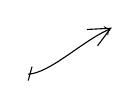
\begin{tikzpicture}[scale=.8]
\draw[->] (0,0) .. controls (.35,.02) and (.85,.52) .. (1.3,.72);
\draw (0,-.10)--(.06,.12);
\draw (.93,.71)--(1.31,.73)--(1.10,.45);
\end{tikzpicture}}

% E537-04
then the homomorphisms induced by $\delta_G$
% E537-05
\[
(33)\qquad
\diagram{\begin{tikzcd}[ampersand replacement=\&,column sep=large]
Z_\rho\arrow[r,"{\delta_\rho}"]\&\gamma_{\rho,\sigma}
\end{tikzcd}},
\qquad
\diagram{\begin{tikzcd}[ampersand replacement=\&,column sep=large]
Z_\sigma\arrow[r,"{\delta_\sigma}"]\&\gamma_{\rho,\sigma}
\end{tikzcd}}
\]
% E537-06
have
% E537-07
\deleted{as}
% E537-08
\inserted{some}
images which contain $\gamma'_{\rho,\sigma}$ and
$\gamma''_{\rho,\sigma}$ respectively,
% E537-09
\deleted{and \unsure{sss|iff} \unsure{to}}

% E537-10
\deleted{Moreover the image of $Z_\rho$ is contained in
$\gamma'_{\rho,\sigma}$
% E537-11
\deleted{if we assume}
% E537-12
\inserted{(\unsure{or equal}) \unsure{sss|iff}}
$\rho$ and $\rho^{-1}$ not conjugate in $\mathcal{G}$,
% E537-13
\deleted{it suffices}
% E537-14
\inserted{and}
% E537-15
\deleted{\unsure{for this}}
likewise the image of $Z_\sigma$ is
\unsure{reduced|reduced} to $\gamma''_{\rho,\sigma}$
\unsure{sss|iff} $\sigma$ and $\sigma^{-1}=-\sigma$
not conjugate in $\mathcal{G}$. Let us note for example
% E537-16
\deleted{that}
% E537-17
\inserted{if}
% E537-18
\deleted{$\mathcal{G}=\mathrm{SL}(2,\widehat{\mathbb{Z}})'$,}
$\sigma^2=1$,
\unsure{the} last condition is not \unsure{satisfied},
hence
% E537-19
$\diagram{\begin{tikzcd}[ampersand replacement=\&]
Z_\sigma\arrow[r]\&\gamma_{\rho,\sigma}
\end{tikzcd}}$
is surjective,
% E537-20
\deleted{it}
% E537-21
\inserted{\deleted{\unsure{but}} it}
is
% E537-22
\deleted{not either}
% E537-23
\deleted{\unsure{that it is satisfied if}}
$\mathcal{G}=\unsure{\mathrm{SL}}(2,\widehat{\mathbb{Z}})$
% E537-24
\inserted{in $\mathrm{SL}(2,\widehat{\mathbb{Z}})$}
$\sigma$ is conjugate there to $-\sigma$, by the
% E537-25
\deleted{(for $\sigma$ and}
general \unsure{theorem} of Steinberg for example) ---
\unsure{can it happen} in the universal \unsure{case}
$\mathrm{SL}(2,\mathbb{Z})^{\wedge}
=\mathcal{G}_{1,1}^{+\wedge}$?
}

% E537-26
\margin{\deleted{
The condition on $\rho$ is not satisfied
% E537-27
\deleted{\unsure{for}}
$\mathcal{G}=\mathrm{SL}(2,\widehat{\mathbb{Z}})/\pm1$,
As in this case the \uline{two} homomorphisms
% E537-28
$\diagram{\begin{tikzcd}[ampersand replacement=\&,column sep=small]
Z_\rho,\deleted{\unsure{Z_\sigma}}\arrow[r]\&
\unsure{\widehat{\gamma}_{\rho,\sigma}|\gamma_{\rho,\sigma}}
=\widehat{\mathbb{Z}}^{*}
\end{tikzcd}}$,
% E537-29
$\diagram{\begin{tikzcd}[ampersand replacement=\&,column sep=small]
Z_\sigma\arrow[r]\&\gamma_{\rho,\sigma}=\widehat{\mathbb{Z}}^{*}
\end{tikzcd}}$
are \unsure{surjections|surjective}),
but it is for $\mathcal{G}=\mathrm{SL}(2,\widehat{\mathbb{Z}})$,
for we find that the image of
% E537-30
$\diagram{\begin{tikzcd}[ampersand replacement=\&,column sep=small]
\unsure{Z_\rho}\arrow[r]\&\gamma_{\rho,\sigma}
\end{tikzcd}}$
is $\gamma'_{\rho,\sigma}$.
But in $\unsure{\mathcal{G}_{0,3}^{+\wedge}}$,
$\rho$ and $\rho^{-1}$ are also not conjugate,
i.e. the image is \unsure{reduced} also to $\gamma'_{\rho,\sigma}$.
}}
% E537-31
\margin{536}

% E537-F01
\margin{\begin{center}
536\\
\texttt{https://grothendieck.umontpellier.fr}\\
Université de Montpellier, UMR CNRS 5149, Case courrier 051, Place Eugène Bataillon\\
34095 Montpellier cedex 5 - France
\end{center}}

\scanpage{538}
% E538-01
\mspage{572}

% E538-02
\uline{Proposition} \quad 1°) The image $\delta_\rho(Z_\rho)$ contains
$\gamma'_{\rho,\sigma}$, and is
% E538-03
\deleted{\unsure{eq}}
% E538-04
reduced to $\gamma'_{\rho,\sigma}$ \unsure{iff|iff}
$\rho$ and $\rho^{-1}$ not conjugate in $\mathcal{G}$ ---
therefore it is equal to $\gamma_{\rho,\sigma}$
i.e.
% E538-05
$\delta_\rho:\diagram{\begin{tikzcd}[ampersand replacement=\&,column sep=large]
Z_\rho\arrow[r]\&\gamma_{\rho,\sigma}
\end{tikzcd}}$
% E538-06
epimorphism \unsure{iff|iff} $\rho$ and $\rho^{-1}$ are conjugate in $\mathcal{G}$.

% E538-07
2°) The image $\delta_\sigma(Z_\sigma)$ contains
$\gamma''_{\rho,\sigma}$, and it is reduced to
$\gamma''_{\rho,\sigma}$ \unsure{iff|iff} $\sigma$ and
$\sigma^{-1}=-\sigma$ not conjugate in $\mathcal{G}$ ---
\unsure{therefore|otherwise} it is equal to $\gamma_{\rho,\sigma}$ i.e.
% E538-08
$\delta_\sigma:\diagram{\begin{tikzcd}[ampersand replacement=\&,column sep=large]
Z_\sigma\arrow[r]\&\gamma_{\rho,\sigma}
\end{tikzcd}}$
% E538-09
epimorphism \unsure{iff|iff} $\sigma$ and
$\unsure{-\sigma^{-1}|\sigma^{-1}}=-\sigma$ are conjugate in $\mathcal{G}$.

% E538-10
\uline{Corollary 1}. If $\mathcal{G}$ contains as a quotient
% E538-11
\[
SL(2,\mathbb{Z}/3\mathbb{Z})',\quad\text{with}\quad
\rho=\begin{pmatrix}0&1\\-1&1\end{pmatrix},\qquad
\sigma=\begin{pmatrix}0&-1\\1&0\end{pmatrix}
\]
% E538-12
$(\bmod\ \pm1)$, then the image of $\delta_\rho$ is
$\gamma'_{\rho,\sigma}$.

% E538-13
Indeed, we see that $\rho$ and $\pm\rho^{-1}$ are not
conjugate in $\mathcal{G}$, for they are
not in $SL(2,\mathbb{Z}/3\mathbb{Z})'$ ---
% E538-14
\deleted{\unsure{for example}\ \unsure{for}}
% E538-15
\inserted{Let us check this:}
% E538-16
$\rho$ and $-\rho^{-1}$ already have distinct traces
$1$ and $-1$, $\unsure{\in}(\mathbb{Z}/3\mathbb{Z})^{\unsure{*}}$,
they are not conjugate.

% E538-17
We have
% E538-18
\[
(\underbrace{\tau\sigma}_{\tau'_\infty})(\rho)=\rho^{-1},
\]
% E538-19
therefore
% E538-26
\deleted{all} the elements of
% E538-20
\deleted{$f\in$}
% E538-21
$GL(2,\mathbb{Z}/3\mathbb{Z})$
% E538-22
\deleted{such that}
% E538-23
which conjugate $\rho$ to $\rho^{-1}$ are of the form
$f\tau'_\infty$, where
% E538-24
$f=\unsure{c|b}\rho+d$, we \unsure{want}
$\det(f\tau'_\infty)=1$ i.e. $\det(f)=-1$
$(\text{since }\det(\tau'_\infty)=-1)$,
i.e. $c^2+\unsure{cd}+d^2=-1$, impossible.
% E538-25
\margin{537}

% E538-F01
\margin{\begin{center}
537\\
\texttt{https://grothendieck.umontpellier.fr}\\
Université de Montpellier, UMR CNRS 5149, Case courrier 051, Place Eugène Bataillon\\
34095 Montpellier cedex 5 - France
\end{center}}

\scanpage{539}

% E539-01
\uline{Corollary 2}\quad If $\sigma^2=1$, then
% E539-02
$\diagram{\begin{tikzcd}[ampersand replacement=\&,column sep=large]
Z_\sigma\arrow[r]\&\gamma_{\rho,\sigma}
\end{tikzcd}}$
% E539-03
is surjective. If On the other hand $\mathcal{G}$ contains as a quotient
% E539-04
\deleted{$\mathbb{Z}/4\mathbb{Z}$}
% E539-05
$SL(2,\mathbb{Z}/4\mathbb{Z})$
$(\uline{\text{without}}\ \prime\ !)$, with $\rho,\sigma$ as
\unsure{usual}, then
% E539-06
\[
\operatorname{Im}(\delta_\sigma)=\gamma''_{\rho,\sigma}.
\]

% E539-07
We must see that $\sigma$ and $\sigma^{-1}=-\sigma$ not conjugate
in $SL(2,\mathbb{Z}/4\mathbb{Z})$, using that
$\tau_\infty(\sigma)=\sigma^{-1}$, therefore
% E539-08
\deleted{it f}
% E539-09
the \unsure{elements|elements} of $GL(2,\mathbb{Z}/4\mathbb{Z})$ which
conjugate $\sigma$ to $\sigma^{-1}$ are the
% E539-10
\inserted{$g=f\tau_\infty$ with}
% E539-11
$f=t\sigma+\unsure{u|n}$,
% E539-12
\deleted{\unsure{with}}
% E539-13
and therefore that $\det(g)=1$ means $\det f=-1$
i.e. $t^2+\unsure{u|n}^2=-1$, impossible.

% E539-14
\deleted{
Let us set
% E539-15
\[
(34)\qquad
\left\{
\begin{aligned}
SZ_\rho&=
% E539-16
\inserted{\operatorname{Ker}\delta_\rho=}
Z_\rho\cap\mathcal{G}=\operatorname{Centr}_{\mathcal{G}}(\rho).\\
SZ_\sigma&=
% E539-17
\inserted{\operatorname{Ker}\delta_\sigma=}
Z_\sigma\cap\mathcal{G}=\operatorname{Centr}_{\mathcal{G}}(\sigma)\\
SB_{\rho,\sigma}&=\operatorname{Ker}\delta_B
=B_{\rho,\sigma}\cap\mathcal{G}=L_0.
\end{aligned}
\right.
\]
}

% E539-18
\deleted{
% E539-19
\[
(35)\qquad
\begin{aligned}
&S_0\unsure{\mathcal{M}|M}_{\rho,\sigma}
\subset B_{\rho,\sigma}\times\unsure{Z_\rho|N_\rho}
\times Z_\sigma\times\unsure{G_{\rho,\sigma}|\gamma_{\rho,\sigma}}\\
&\text{''}\\
&\bigl\{(u,a,b,U\unsure{\}|)}\ \bigm|\,
\delta_B(u)=\delta_G(U)=\delta_\sigma(b)
=\varepsilon_3(\mu)\delta_\rho(a)\bigr\}
\end{aligned}
\]
}
% E539-20
\margin{538}

% E539-F01
\margin{\begin{center}
538\\
\texttt{https://grothendieck.umontpellier.fr}\\
Université de Montpellier, UMR CNRS 5149, Case courrier 051, Place Eugène Bataillon\\
34095 Montpellier cedex 5 - France
\end{center}}

\scanpage{540}
% E540-01
\mspage{573}

% E540-02
% E540-03
Let us note that by (2), \inserted{(4)}, we have
% E540-04
\[
(35)\qquad \tau_B \overset{\mathrm{dfn}}{=}(\tau,-1)\in B_{\rho,\sigma}
\]
% E540-05
And obviously $\tau_B\notin L_0=B_{\rho,\sigma}\cap\mathcal{G}$.
So we have an embedding
% E540-06
\[
(36)\qquad
\left\{
\begin{array}{l}
\diagram{\begin{tikzcd}[ampersand replacement=\&,column sep=large,row sep=small]
\mathcal{G}'=\{1,\tau\}.\mathcal{G} \arrow[r,hook] \& G_{\rho,\sigma}\\
\tau \arrow[r,mapsto] \& \tau_B\\
g \arrow[r,mapsto] \& g\quad\text{if }g\in\mathcal{G}
\end{tikzcd}}
\end{array}
\right.,
\]
% E540-07
\margin{\uline{N.B.} $\mathcal{G}'$ is a quotient of
$\mathrm{GL}(2,\mathbf{Z})^\wedge$, and $\tau$ corresponds there to
the image of the element
$\tau_\infty=\begin{pmatrix}-1&0\\0&1\end{pmatrix}$
of $\unsure{\mathrm{GL}(2,\mathbf{Z})}$.}

% E540-08
% E540-09
therefore the \unsure{automorphism} $\tau$ of $\mathcal{G}$ will be considered as
induced by \deleted{\unsure{the ele}} $\operatorname{int}(\tau_B)$,
where $\tau_B$ is itself considered as an
element of $G_{\rho,\sigma}$.

% E540-10
% E540-11
\deleted{\illegible{2}} In connection with the equality
% E540-12
\[
\tau_B(\sigma)=\sigma^{-1}\quad(=-\sigma)
\]
% E540-13
% E540-14
% E540-15
% E540-16
% E540-18
% E540-17
which shows that $\tau_B$ normalizes the subgroup
\inserted{$L_\sigma$} \inserted{generated by $\sigma$}
(isomorphic to a quotient of $\mathbf{Z}/4\mathbf{Z}$),
\deleted{\unsure{group}} \inserted{therefore}
\inserted{normalizes $Z_\sigma=\operatorname{Centr}_{G_{\rho,\sigma}}(L_\sigma)$},
\deleted{\unsure{then let us introduce}} let us introduce
% E540-19
\[
(37)\qquad
N_\sigma=\underset{(\text{$1/2$ direct})}{\{1,\tau_B\}.Z_\sigma},
\]
% E540-20
and the canonical homomorphism
% E540-21
\[
(38)\qquad
\left\{
\begin{array}{l}
\diagram{\begin{tikzcd}[ampersand replacement=\&,column sep=large,row sep=small]
N_\sigma \arrow[r,"i_\sigma"] \& G_{\rho,\sigma} \& \&\\
\tau_B \arrow[r,mapsto] \& \tau_B, \& x \arrow[r,mapsto] \& x\quad\text{if }x\in Z_\sigma
\end{tikzcd}}
\end{array}
\right..
\]

% E540-22
\deleted{This homomorphism is injective iff}
% E540-23
% E540-24
The image of this homomorphism is none other than the normalizer of $\sigma$
in $G_{\rho,\sigma}$, for a \deleted{\unsure{automorphism}}
$g\in G_{\rho,\sigma}$ which normalizes $L_\sigma$ must transform
$\sigma$ into a generator of $L_\sigma$, i.e. into $\sigma$ or
$\sigma^{-1}$, in the first case we will have $g\in Z_\sigma$, in
the second $g(\sigma)=\tau_B(\sigma)$ i.e. $\tau_B^{-1}g\in Z_\sigma$
i.e. $g\in\tau_B Z_\sigma$. The homomorphism (38) is injective

% E540-25
\margin{539}

% E540-F01
\margin{\begin{center}
539\\
\texttt{https://grothendieck.umontpellier.fr}\\
Université de Montpellier, UMR CNRS 5149, Case courrier 051, Place Eugène Bataillon\\
34095 Montpellier cedex 5 - France
\end{center}}

\scanpage{541}
% E541-01
\deleted{iff $\tau_B\in Z$}
% E541-02
iff $\tau_B\notin Z_\sigma$ i.e. $\sigma\ne\sigma^{-1}$ i.e.
$\sigma^2\ne1$ i.e. ``$-1$'' $\ne1$.

% E541-03
While we are at it, let us take advantage of the formula
% E541-04
\[
\tau_B(\rho)=\sigma(\rho^{-1})
\]
% E541-05
to introduce
% E541-06
\[
(39)\qquad
\tau'\uuline{=}\sigma^{-1}\tau\in\mathcal{G}'\subset G_{\rho,\sigma}
\]
% E541-07
(which corresponds to the element
% E541-08
% E541-09
\[
(40)\qquad
\tau'_\infty=\sigma_\infty^{-1}\tau_\infty
=-\sigma_\infty\tau_\infty
=\begin{pmatrix}0&1\\1&0\end{pmatrix}
\in\underbrace{\mathrm{GL}(2,\mathbf{Z})}_{
\inserted{\substack{\Vert\\\mathcal{T}_{1,1}}}}
\biggr),
\]

% E541-10
% E541-11
\deleted{\unsure{which is}} we will therefore have
% E541-12
\[
(40)\qquad \tau'^2=1,\qquad \tau'(\rho)=\rho^{-1}.
\]

% E541-13 deletion
\deleted{Let us therefore introduce}
% E541-14 deletion
\deleted{$(41)\qquad N_\rho=\{1,\tau'\}.$}
% E541-15
% E541-16
\inserted{Thus $\tau'$ normalizes the subgroup $L_\rho$
(isomorphic to a quotient of $\mathbf{Z}/6\mathbf{Z}$) generated
by $\rho$, therefore it normalizes the centralizer
\inserted{$Z_\rho$} of $L_\rho$, and we can construct}
% E541-17
% E541-18
\margin{\uline{N.B.} We have at the same time
$\tau'(\sigma)=\sigma^{-1}$, therefore we can consider $\tau'$
as an element of $N_\sigma$, and \deleted{\illegible{1}} we have
$N_\sigma=\{1,\tau'\}.Z_\sigma$ (which is $1/2$ direct)}
% E541-19
\[
(41)\qquad
N_\rho\overset{\mathrm{dfn}}{=}
\underset{(\text{semidirect})}{\{1,\tau'\}.Z_\rho}
\]
% E541-20
% E541-21
% E541-22
and \deleted{\unsure{a}} \deleted{\unsure{of the}} canonical homomorphism
% E541-23
\[
(42)\qquad
\left\{
\begin{array}{l}
\diagram{\begin{tikzcd}[ampersand replacement=\&,column sep=large,row sep=small]
N_\rho \arrow[r,"i_\rho"] \& G_{\rho,\sigma} \& \&\\
\tau' \arrow[r,mapsto] \& \tau', \& x \arrow[r,mapsto] \& x\quad\text{for }x\in Z_\rho
\end{tikzcd}}
\end{array}
\right..
\]

% E541-24
% E541-25
% E541-26
% E541-27
The image of this homomorphism is the normalizer of $L_\rho$ in
$G_{\rho,\sigma}$ --- we see this as \unsure{a moment ago} for $i_\sigma$,
noting that \deleted{the}
\inserted{$\rho,\rho^{-1}$ are the \uline{only}} generators of
$L_\rho$. The homomorphism $i_\rho$ is injective iff $\tau'\notin Z_\rho$
i.e. \deleted{\unsure{iff}} $\rho\ne\rho^{-1}$ i.e. $\rho^2\ne1$
i.e. $\rho\ne-1$
% E541-28
% E541-29
% E541-30
% E541-31
% E541-32
(\deleted{\unsure{in this case}}
\inserted{N.B. \uline{$\rho=-1$}}
\deleted{\unsure{implies}} \deleted{\unsure{equivalent}}
\deleted{\unsure{in fact}} that $\rho$ commutes with $\sigma$, and that
$\mathcal{G}$ is a quotient of $\mathbf{Z}/12\mathbf{Z}$, with
$\rho$ corresponding to $2$
% E541-33 insertion
\inserted{and $\sigma$ to $3$, but here $2\rho=0$ therefore
$\mathcal{G}$ is a quotient of $\mathbf{Z}/4\mathbf{Z}$ with
$\rho$ corresponding to $2$, $\sigma$ to $3=-1\ldots$}).

% E541-34
% E541-35
\margin{
\[
(43)\qquad\left\{
\begin{array}{l}
\diagram{\begin{tikzcd}[ampersand replacement=\&,column sep=huge,row sep=large]
N_\rho \arrow[r,"\delta_\rho=\delta_G\circ i_\rho"] \& \gamma_{\rho,\sigma}\\
N_\sigma \arrow[r,"\delta_\sigma=\delta_G\circ i_\sigma"] \& \gamma_{\rho,\sigma}
\end{tikzcd}}\\
\hfill\text{epimorphisms}
\end{array}
\right.
\]}
% E541-36
\margin{``We have done what was needed'' to have
\uline{epimorphisms} $\unsure{\varphi}$.}
% E541-37
\margin{540}

% E541-F01
\margin{\begin{center}
540\\
\texttt{https://grothendieck.umontpellier.fr}\\
Université de Montpellier, UMR CNRS 5149, Case courrier 051, Place Eugène Bataillon\\
34095 Montpellier cedex 5 - France
\end{center}}

\scanpage{542}
\mspage{574}
% E542-01
\deleted{\(\unsure{(43)}\)}
% E542-02
\unsure{Let us situate|Let}
% E542-03
\deleted{\(\unsure{\mathfrak{g}|g}\)}

% E542-04
\[
(44)\qquad
\begin{gathered}
S\unsure{\mathfrak{g}|g}_{\rho,\sigma}^{\unsure{*}}
\subset \mathcal{G}'\times\mathcal{G}\times\widehat{\mathbb Z}^{*}
\\[-2pt]
\Vert\\[-2pt]
\left\{(\alpha,\beta,\mu)\ \left|
\begin{array}{l}
\alpha\equiv\tau^{\nu_3(\mu)}\bmod\mathcal{G}
\quad\text{i.e. }\chi(\alpha)=\varepsilon_3(\mu)\\
\underbrace{\alpha\rho(\alpha)^{-1}}_{\zeta}
=\underbrace{\varepsilon_2(\mu)\beta\sigma(\beta)^{-1}}_{\eta}
\ell_1^\nu,\quad\text{where}
\end{array}\right.\right\}
\end{gathered}
\]
% E542-05
\inserted{\[
\nu=(\mu-1)/2,\qquad\uline{(\ell_1=\varepsilon_1^2)}
\]}

% E542-06
\deleted{\[
(\unsure{36})\qquad
\unsure{\mathfrak{g}|g}_{\rho,\sigma}^{\unsure{*}\,\mathrm{eff}}
=\left\{(\alpha,\beta,\mu)\in
\unsure{\mathfrak{g}|g}_{\rho,\sigma}^{*}\ \middle|\ \unsure{\exists}\right.
\]}

% E542-07
whence

% E542-08
% E542-09
\begin{samepage}
\[
(45)
\]
\diagram{\(
\left\{
\begin{gathered}
\begin{tikzcd}[ampersand replacement=\&,column sep=large]
S\unsure{\mathfrak{g}|g}_{\rho,\sigma}^{\unsure{*}}
\arrow[r] \&
\begin{gathered}
\Sigma_{\rho,\sigma}\subset\mathcal{G}\times\mathcal{G}\times\widehat{\mathbb Z}^{*}\\[-2pt]
\Vert\quad\mathrm{dfn}\\[-2pt]
\left\{(\zeta,\eta,\mu)\ \left|
\begin{array}{l}
\zeta\rho\ \text{conjugation in }\mathcal{G}:\rho^\mu\\
\unsure{\eta|\zeta}\sigma\quad\underline{\hspace{7em}}\quad\sigma^\mu\\
\zeta=\deleted{\unsure{\beta\sigma(\beta)^{-1}}}\eta\ell_1^\nu
\end{array}\right.\right.
\end{gathered}\\
(\alpha,\beta,\mu)\arrow[r,mapsto]\&
\left(\overbrace{\alpha\rho(\alpha)^{-1}}^{[\alpha,\rho]},
\varepsilon_2(\mu)\overbrace{\beta\sigma(\beta)^{-1}}^{[\beta,\sigma]},\mu\right).
\end{tikzcd}
\end{gathered}
\right.
\)}
\end{samepage}
% E542-10
\inserted{\((\text{where }\nu=(\mu-1)/2\)}
% E542-11
We denote by
\(\unsure{\mathfrak{g}|g}_{\rho,\sigma}^{\unsure{*}\,\mathrm{eff}}\)
the inverse image of
\(\Sigma_{\rho,\sigma}^{\mathrm{eff}}\)
(cf. corollary page 570). \(\simeq B_{\rho,\sigma}\).
By \unsure{construction}
% E542-12
\inserted{we thus find a \uline{surjective} map}
% E542-13
\margin{
\((\unsure{46\mathrm{bis}})\)
\diagram{\begin{tikzcd}[ampersand replacement=\&]
S\unsure{\mathfrak{g}|g}_{\rho,\sigma}^{\mathrm{eff}}
\arrow[r,"\text{epimorphism}"]\&[30pt]
\Sigma_{\rho,\sigma}^{\mathrm{eff}}
\end{tikzcd}}
}

% E542-14
We regard
\(S\unsure{\mathfrak{g}|g}_{\rho,\sigma}^{*}\)
as contained in a
% E542-15
\deleted{group}
% E542-16
\inserted{set}
% E542-17
that is larger

% E542-18
% E542-19
\[
(47)\qquad
\begin{gathered}
\unsure{\mathfrak{g}|g}_{\rho,\sigma}^{\unsure{*}}
\subset G_{\rho,\sigma}\times G_{\rho,\sigma}
\times\widehat{\mathbb Z}^{*}
\\[-2pt]
\Vert\\[-2pt]
\left\{(\alpha,\beta,\mu)\ \left|
\begin{array}{l}
\chi(\alpha)\equiv\varepsilon_3
\bigl(\deleted{\unsure{\chi(\mu)|\chi(\beta)}}\mu\bigr)
\chi(\beta);\\
\underbrace{\alpha\rho(\alpha)^{-1}}_{=\alpha(\rho)\rho^{-1}=\zeta}
=
\underbrace{\varepsilon_2(\mu)\beta\sigma(\beta)^{-1}}_
{=\varepsilon_2(\mu)\beta(\sigma)\sigma^{-1}=\eta}
\ell_1^\nu
\end{array}\right.\right\}
\end{gathered}
\]
% E542-20
so that we will have
% E542-21
% E542-22
\[
(48)\qquad
\begin{aligned}
S\unsure{\mathfrak{g}|g}_{\rho,\sigma}^{\unsure{*}}
&=\unsure{\mathfrak{g}|g}_{\rho,\sigma}^{\unsure{*}}
\cap\bigl(\mathcal{G}'\times\mathcal{G}\times\widehat{\mathbb Z}^{*}\bigr),
\\
&=\left\{(\alpha,\beta,\mu)\in
\unsure{S\mathfrak{g}|Sg}_{\rho,\sigma}^{*}
\ \left|
\begin{array}{l}
\delta_\sigma(\beta)=1\deleted{\unsure{\}}}\\
\delta_\rho\bigl(\alpha\tau^{\nu_3(\mu)}\bigr)=1
\end{array}\right.\right\}
\end{aligned}
\]
% E542-23
\margin{541}

% E542-F01
\margin{\begin{center}
541\\
\texttt{https://grothendieck.umontpellier.fr}\\
Université de Montpellier, UMR CNRS 5149, Case courrier 051, Place Eugène Bataillon\\
34095 Montpellier cedex 5 - France
\end{center}}

\scanpage{543}
% E543-01
and we again have a canonical map
% E543-02
\begin{samepage}
\[
(49)
\]
\diagram{\(
\left\{
\begin{gathered}
\begin{tikzcd}[ampersand replacement=\&,column sep=large]
\unsure{\mathfrak{g}|g}_{\rho,\sigma}^{*}\arrow[r]\&
\Sigma_{\rho,\sigma}^{\unsure{*}}\\
(\alpha,\beta,\mu)\arrow[r,mapsto]\&
\bigl([\alpha,\rho],\varepsilon_2(\mu)[\beta,\sigma],\mu\bigr).
\end{tikzcd}
\end{gathered}
\right.
\)}
\end{samepage}

% E543-03
\deleted{\unsure{whose i}}
% E543-04
We denote by
\(\unsure{\mathfrak{g}|g}_{\rho,\sigma}^{\mathrm{eff}}\)
the inverse image of
\(\Sigma_{\rho,\sigma}^{\mathrm{eff}}\),
and we find
% E543-05
\[
(50)\qquad
\begin{aligned}
S\unsure{\mathfrak{g}|g}_{\rho,\sigma}^{\mathrm{eff}}
&=\unsure{\mathfrak{g}|g}_{\rho,\sigma}^{\mathrm{eff}}
\cap\bigl(\mathcal{G}'\times\mathcal{G}\times\widehat{\mathbb Z}^{*}\bigr)
\\
&=\left\{(\alpha,\beta,\mu)\in
\unsure{\mathfrak{g}|g}_{\rho,\sigma}^{\mathrm{eff}}
\ \left|
\begin{array}{l}
\delta_\sigma(\beta)=1\\
\unsure{\delta_\rho|\delta_B}\bigl(\alpha{\tau'}^{\nu_3(\mu)}\bigr)=1
\end{array}\right.\right\}
\end{aligned}
\]

% E543-06
We have a section of
% E543-07
% E543-08
% E543-09
% E543-10
\begin{samepage}
\[
(51)
\]
\diagram{
\begin{tikzcd}[ampersand replacement=\&,column sep=large,row sep=large]
\unsure{\mathfrak{g}|g}_{\rho,\sigma}^{\mathrm{eff}}\arrow[r]\&
\Sigma_{\rho,\sigma}^{\mathrm{eff}}\&
\zeta=[u,\rho],\overset{\inserted{\eta=}}{[u,\sigma]},
\overset{\inserted{\mu=}}{\chi_B(u)}
\\
\& B_{\rho,\sigma}
\arrow[u,"\sim"']
\arrow[ul,"\text{\uline{section}}"]\&
u\deleted{\unsure{\varphi|*}}\arrow[u,mapsto]
\end{tikzcd}
}
\end{samepage}

% E543-11
given by
% E543-12
% E543-13
% E543-14
\begin{samepage}
\[
(52)
\]
\diagram{\begin{tikzcd}[ampersand replacement=\&,column sep=large]
u\deleted{\unsure{\varphi|*}}\arrow[r,mapsto]\&
\bigl(\deleted{\unsure{\alpha=}}u,\,
u{\tau'}^{\nu_2(\mu)},\,\mu=\chi_B(u)\bigr)
\end{tikzcd}}
\end{samepage}

% E543-15
since we will have
(setting \(\varepsilon=\varepsilon_2(\mu)
\unsure{\overset{\mathrm{dfn}}{=}|=}
(-1)^{\nu_2}\).)
% E543-16
\[
[u,\rho]=u\rho(u)^{-1}=\zeta
\]
% E543-17
\[
\begin{aligned}
\varepsilon
\left[u{\tau'}^{\nu_2(\mu)=\nu_2},\sigma\right]
&=\varepsilon u{\tau'}^{\nu_2}
\sigma\bigl(u\unsure{\tau|\tau'}^{\nu_2}\bigr)^{-1}\\
&=\varepsilon u
\left(\underbrace{
\unsure{\tau|\tau'}^{\nu_2}
\sigma\bigl(\unsure{\tau|\tau'}^{\nu_2}\bigr)^{-1}
}_{=\varepsilon}\right)\sigma(u)^{-1}
=\unsure{\varepsilon u|u}\sigma(u)^{-1}=\eta
\end{aligned}
\]
% E543-18
OK. So
% E543-19
\deleted{\unsure{the set|the}}
% E543-20
% E543-21
\inserted{the set \deleted{\unsure{of the}}
\(\unsure{\mathfrak{g}_{\rho,\sigma}(u,\mu)|g_{\rho,\sigma}^{(u,\mu)}}\)}
% E543-27
of the \((\alpha,\beta,\mu)\,\unsure{-}\)
giving \unsure{the image}
% E543-22
% E543-23
% E543-24
\[
(\zeta,\eta,\mu)\deleted{\unsure{\Longrightarrow|=}}
\unsure{[|(}\,[u,\rho],[u,\sigma],
\overset{\inserted{\mu=}}{\chi_B(u)}\bigr)
\]
% E543-25
\unsure{will be exactly}
% E543-26
\margin{542}

% E543-F01
\margin{\begin{center}
542\\
\texttt{https://grothendieck.umontpellier.fr}\\
Université de Montpellier, UMR CNRS 5149, Case courrier 051, Place Eugène Bataillon\\
34095 Montpellier cedex 5 - France
\end{center}}

\scanpage{544}
\mspage{575}
% E544-01
\deleted{\unsure{the}}
% E544-02
\inserted{\(
\unsure{\mathfrak{g}_{\rho,\sigma}(u,\mu)|g_{\rho,\sigma}^{(u,\mu)}}
=
\)}
% E544-03
\[
(53)\qquad
\left\{\left(
\overbrace{ua_0^{-1}}^{\alpha},
\overbrace{u{\tau'}^{\nu_2}b_0^{-1}}^{\unsure{\beta|b}},
\mu\right)
\ \middle|\ a_0\in Z_\rho,\ b_0\in Z_\sigma,\
\nu_2=\nu_2(\mu)\right\}
\]
% E544-04
\inserted{\[
\bigl(=(ua_0^{-1},ub^{-1},\mu)\unsure{\}}
\quad\text{where}\quad b=b_0{\tau'}^{\unsure{\nu_2}}
\]}
% E544-05
which we also write
% E544-06
% E544-29
\[
(54)\qquad
\unsure{\mathfrak{g}_{\rho,\sigma}(u,\mu)|g_{\rho,\sigma}^{(u,\mu)}}
=
\left\{\left(
\underbrace{ua_0^{-1}}_{\alpha},
\underbrace{u\,i_\sigma(b)}_{\beta},
\mu\right)
\ \middle|\ 
a_0\in Z_\rho,\ 
\underset{\inserted{\text{(cf. (37)(38))}}}{b\in N_\sigma},\
\boxed{\varepsilon_\sigma(b)=\varepsilon_2(\mu)}
\right\}
\]
% E544-07
where \(\varepsilon_\sigma:N_\sigma\longrightarrow\{\pm1\}\)
is defined in (37) as the canonical homomorphism
fitting into the exact sequence
% E544-08
\begin{samepage}
\[
(55)
\]
\diagram{\begin{tikzcd}[ampersand replacement=\&]
1\arrow[r]\&Z_\sigma\arrow[r]\&N_\sigma
\arrow[r,"\varepsilon_\sigma"]\&
\underbrace{\{\pm1\}}_{\simeq\{1,\tau'\}}\arrow[r]\&1.
\end{tikzcd}}
\end{samepage}

% E544-09
If we look for the set of elements of
\(S\unsure{\mathfrak{g}|g}_{\rho,\sigma}^{\mathrm{eff}}\)
over \((\zeta,\eta,\mu)\), we must in addition
impose the conditions
% E544-10
\[
(56)\qquad
\deleted{\unsure{\alpha=}}ua_0^{-1}{\tau'}^{\nu_3(\mu)}\in\mathcal{G},
\quad u\,i_\sigma(b)\in\mathcal{G}
\]
% E544-11
i.e.
\[
\delta_G(ua_0^{-1}{\tau'}^{\nu_3})=1,\quad
\delta_G(u\,i_\sigma(b))=1
\]
% E544-12
that is, again
% E544-13
\[
(57)\qquad
\delta_G(u)=
\underbrace{\delta_\sigma(b)}_{\text{cf. (43)}}
=
\underbrace{\delta_\rho}_{\text{cf. (43)}}
({\tau'}^{\nu_3}.a_0).
\]
% E544-14
Let us therefore set
\[
a={\tau'}^{\nu_3}.a_0\quad\text{\unsure{in|in}}\ N_\rho
\]
% E544-15
\inserted{\((\text{thus }a_0={\tau'}^{\nu_3}a)\)}
% E544-16
we see that
% E544-17
\[
(54)\qquad
\unsure{\mathfrak{g}_{\rho,\sigma}(u,\mu)|g_{\rho,\sigma}^{(u,\mu)}}
=
\left\{(ua^{-1}{\tau'}^{\nu_3},ub^{-1},\mu)\ \left|
\begin{array}{l}
a\in N_\rho,\ b\in N_\sigma\ \text{such that}\\
\varepsilon_\rho(a)=\varepsilon_3(\mu),\
\varepsilon_\sigma(b)=\varepsilon_2(\mu)\\
\delta_\rho(a)=\delta_\sigma(b)=\delta_G(u)
\end{array}\right.\right\}
\]

% E544-18
Let us therefore introduce the group
% E544-19
% E544-20
\[
(55)\qquad
\deleted{\unsure{S_0}}
\unsure{\mathcal{M}|M}_{\rho,\sigma}[0]
=\unsure{B}_{\rho,\sigma}
\times_{\gamma_{\rho,\sigma}}N_\rho
\times_{\gamma_{\rho,\sigma}}N_\sigma.
\]
% E544-21
and the composite homomorphisms
% E544-22
% E544-23
% E544-24
\begin{samepage}
\[
(56)
\]
\diagram{\(
\left\{
\begin{gathered}
\begin{tikzcd}[ampersand replacement=\&,column sep=large]
\deleted{\unsure{S_0}}\unsure{\mathcal{M}|M}_{\rho,\sigma}[0]
\arrow[r]\&N_\rho\&
\overset{\varepsilon_\rho}{\unsure{\longleftrightarrow|\longrightarrow}}\&
\{\pm1\}
\\
\deleted{\unsure{S_0}}\unsure{\mathcal{M}|M}_{\rho,\sigma}[0]
\arrow[r]\&N_\sigma\arrow[rr,"\varepsilon_\sigma"]\&\&
\{\pm1\}
\end{tikzcd}
\end{gathered}
\right.
\)}
\end{samepage}
% E544-25
% E544-28
\margin{\deleted{\unsure{denoted}\ \(\varepsilon'_\rho\)}}
% E544-26
(again denoted \(\varepsilon_\rho,\varepsilon_\sigma\)
by abuse of notation)
% E544-27
\margin{543}

% E544-F01
\margin{\begin{center}
543\\
\texttt{https://grothendieck.umontpellier.fr}\\
Université de Montpellier, UMR CNRS 5149, Case courrier 051, Place Eugène Bataillon\\
34095 Montpellier cedex 5 - France
\end{center}}

\scanpage{545}
% E545-01
and

% E545-02
% E545-03
\begin{samepage}
\noindent(57)\quad
\diagram{\begin{tikzcd}[ampersand replacement=\&,column sep=large]
\deleted{\unsure{S_0}}M_{\rho,\sigma}[0]
  \arrow[r,"\delta_{SM}"]
\& \gamma_{\rho,\sigma} \arrow[r,"\chi_\gamma"]
\& \widehat{\mathbb Z}^{*}
\end{tikzcd}}
\end{samepage}
i.e. $\chi_{SM}$, (or \unsure{simply|simply} $\chi$)

% E545-04
consider

% E545-05
% E545-06
\begin{samepage}
\noindent(58)\quad
\diagram{\begin{tikzcd}[ampersand replacement=\&,column sep=huge]
\deleted{\unsure{S_0}}M_{\rho,\sigma}[0]
 \arrow[r,"{\varepsilon_{\rho,\sigma}=(\unsure{\varepsilon_\sigma},\varepsilon_\rho)}"{yshift=3pt}]
\& \{\pm1\}\times\{\pm1\}
\end{tikzcd}}
\end{samepage}

% E545-07
and

% E545-08
% E545-09
\begin{samepage}
\noindent(59)\quad
\diagram{\begin{tikzcd}[ampersand replacement=\&,column sep=huge]
\deleted{\unsure{S_0}}M_{\rho,\sigma}[0]
 \arrow[r,"{\varepsilon_{2,3}:x\longmapsto(\unsure{\varepsilon_2}(\chi(x)),\varepsilon_3(\chi(x)))}"]
\&[85pt] \{\pm1\}\times\{\pm1\}
\end{tikzcd}}
\end{samepage}

% E545-10
and consider the subgroup of coincidences of the two preceding homomorphisms

% E545-11
% E545-12
% E545-13
% E545-14
\[
\begin{aligned}
(60)\quad
\deleted{\unsure{S_0}}M_{\rho,\sigma}^{\unsure{\mathrm{eff}}}[0]
 &\overset{\mathrm{dfn}}=
 \{x\in\unsure{S_0\{M_{\rho,\sigma}\}}\mid
 \varepsilon_{\rho,\sigma}(x)=\varepsilon_{2,3}(x)\}
\\
 &=\left\{\left(
 \underset{\substack{\rotatebox{90}{$\in$}\\ B_{\rho,\sigma}}}{u},
 \underset{\substack{\rotatebox{90}{$\in$}\\ N_\rho}}{a},
 \underset{\substack{\rotatebox{90}{$\in$}\\ Z_\sigma}}{b}
 \right)\ \middle|\
 \begin{gathered}
 \delta_B(u)=\delta_\rho(a)=\delta_\sigma(b)
 \quad\text{i.e. }\Delta\in\gamma_{\rho,\sigma}\\
 \varepsilon_\rho(a)=
 \deleted{\unsure{\varepsilon_3(\chi_B(u))}}
 \inserted{\varepsilon_3(\chi_\gamma(\Delta))},
 \quad\varepsilon_\sigma(b)=\varepsilon_2(\chi_\gamma(\Delta))
 \end{gathered}
 \right.
\end{aligned}
\]

% E545-15
We have a natural map

% E545-16
\begin{samepage}
\noindent(61)\quad
\diagram{\begin{tikzcd}[ampersand replacement=\&,column sep=huge]
M_{\rho,\sigma}^{\mathrm{eff}}[0] \arrow[r]
 \& \mathcal G'\times\mathcal G\times\widehat{\mathbb Z}^{*}\\
(u,a,b)\arrow[r,mapsto] \& (\alpha,\beta,\mu)
\end{tikzcd}}
\end{samepage}
, with
$\begin{gathered}
\alpha=ua^{-1}\tau'^{\nu_\rho(a)}\\
\beta=ub^{-1}\\
\mu=\chi_B(u)=\chi_\rho(a)=\chi_\sigma(b)
\end{gathered}$

% E545-17
\margin{\uline{N.B.} we have identified $a\in N_\rho$, $b\in N_\sigma$
\unsure{with their images} $i_\rho(a)$, $i_\sigma(b)$ in $G_{\rho,\sigma}$.}

% E545-18
% E545-19
\margin{\uline{N.B.} We have set \deleted{\unsure{(61)}}
$\nu_\rho(a)\in\mathbb Z/2$ such that
$(-1)^{\nu_\rho(a)}=\varepsilon_\rho(a)$}

% E545-20
and we have done what was needed for it to be \unsure{injective}
and have as image $S\unsure{\mathfrak{g}|g}_{\rho,\sigma}^{\mathrm{eff}}$, hence induce a bijection

% E545-21
\begin{samepage}
\noindent(62)\quad
\diagram{\begin{tikzcd}[ampersand replacement=\&,column sep=large]
M_{\rho,\sigma}^{\mathrm{eff}}[0] \arrow[r,"\sim"]
 \& S\unsure{\mathfrak{g}|g}_{\rho,\sigma}^{\mathrm{eff}}.
\end{tikzcd}}
\end{samepage}

% E545-22
% E545-23
\uline{Remark}. In fact \inserted{the formulas for} (61)
\unsure{define} even a map

% E545-24
\begin{samepage}
\noindent(62)\quad
\diagram{\begin{tikzcd}[ampersand replacement=\&,column sep=large]
M_{\rho,\sigma}[0]\arrow[r]
\&\mathcal G'\times\mathcal G\times\widehat{\mathbb Z}^{*}
\end{tikzcd}}
\end{samepage}

% E545-25
and for a $(u,a,b)\in M_{\rho,\sigma}[0]$, its image $(\alpha,\beta,\mu)$
is related to $u\in B_{\rho,\sigma}$ by the formulas

% E545-26
\margin{544}

% E545-F01
\margin{\begin{center}
544\\
\texttt{https://grothendieck.umontpellier.fr}\\
Université de Montpellier, UMR CNRS 5149, Case courrier 051, Place Eugène Bataillon\\
34095 Montpellier cedex 5 - France
\end{center}}

\scanpage{546}
\mspage{576}

% E546-01
% E546-02
% E546-03
\[
(63)\quad
\left\{\begin{aligned}
u(\rho)&=\operatorname{int}(\alpha)(\rho)
&&\bigl(\inserted{\mathcal G-}\text{conjugate to }\rho^{\unsure{\varepsilon'}},
\text{ where }\varepsilon'=\varepsilon_\rho(a)\bigr)\\
u(\sigma)&=\varepsilon\operatorname{int}(\beta)(\sigma)
&&\bigl(\mathcal G\text{-conjugate to }\sigma^\varepsilon,
\text{ where }\varepsilon=\varepsilon_\sigma(b)\bigr)\\
&\deleted{\unsure{\alpha}}
\end{aligned}\right.
\]

% E546-04
(but without necessarily having
$\varepsilon'=\varepsilon_3(\mu)$, $\varepsilon=\varepsilon_2(\mu)$).

% E546-05
% E546-06
This suggests a definition of a group a little bigger than $B_{\rho,\sigma}$,
in which $B_{\rho,\sigma}$ \unsure{will be} \inserted{included}
as a \unsure{normal|$\triangleleft$} subgroup \unsure{of index|of index}
$1,2$ or $4$ --- and which will have the advantage, in the ``good cases'', of being the group
of adelic points of a \unsure{suitable} group scheme over $\mathbb Z$.

% E546-07
% E546-08
On the other hand, to \deleted{\unsure{kill}} eliminate the sign
$\varepsilon$ in (63), (which is present \unsure{even} if
$(u,a,b)\in M_{\rho,\sigma}[0]^{\mathrm{eff}}$), I feel like replacing $\beta$ by

% E546-09
\deleted{$\unsure{\beta'}=\tau'^{\nu}\beta'$, where
$\nu\in\mathbb Z/2$ \unsure{is related}}

% E546-10
\[
(64)\quad \beta'=\tau'^{\nu}\beta
\qquad\left(\text{where }\nu\in\mathbb Z/2\mathbb Z\text{ related by }
(-1)^\nu=\varepsilon\right)
\]

% E546-11
So that we will have

% E546-12
\[
(65)\quad \deleted{\unsure{\varepsilon|\chi}}u(\sigma)=\operatorname{int}(\beta')(\sigma)
\quad\text{i.e.}\quad [u,\sigma]=\beta'\sigma(\beta')^{-1}.
\]

% E546-13
This is related to the convention \unsure{that a|which a}
$u\in\Gamma_{\mathbb Q}^{\sim}$, which we were specifying by the pair
$(\alpha,\beta)\in\widehat{\Pi}_{0,3}'\times\widehat{\Pi}_{0,3}$,
will henceforth be specified by the pair
$(\alpha,\beta')\in\widehat{\Pi}_{0,3}\times\widehat{\Pi}_{0,3}'$, with

% E546-14
\[
(66)\quad\unsure{\chi}(\alpha)=\varepsilon_3(\mu),
\quad\chi(\beta')=\varepsilon_2(\mu)
\qquad\bigl(\text{where }\mu=\chi(u)\text{ is the multiplier}\bigr)
\]

% E546-15
% E546-16
% E546-17
which \deleted{gives} for the operation of $u$ on
\deleted{$\unsure{\mathcal G_{0,3}^{+\wedge}}$}

% E546-18
\[
\mathcal G_{0,3}^{+\wedge}
=\mathrm{SL}(2,\mathbb Z)^{\wedge\unsure{\text{\textcircled{1}}}}
=\mathrm{SL}(2,\mathbb Z)^{\wedge}/\pm1
\]

% E546-19
does not in fact change the particular formulas:

% E546-20
% E546-21
\[
(67)\quad\left\{\begin{aligned}
u(\rho)&=\operatorname{int}(\alpha).\rho,\quad
u(\sigma)=\operatorname{int}(\beta)\sigma
\quad(=\operatorname{int}(\beta').\sigma)\\
\alpha\rho(\alpha)^{-1}
&=\beta\underset{\deleted{\unsure{\varepsilon}}}{\unsure{\sigma}}(\beta)^{-1}\ell_1^\nu
\quad(=\beta'\sigma(\beta')^{-1}\ell_1^\nu)
\end{aligned}\right.
\qquad\nu=\frac{\mu-1}{2}
\]

% E546-22
\margin{545}

% E546-F01
\margin{\begin{center}
545\\
\texttt{https://grothendieck.umontpellier.fr}\\
Université de Montpellier, UMR CNRS 5149, Case courrier 051, Place Eugène Bataillon\\
34095 Montpellier cedex 5 - France
\end{center}}

\scanpage{547}

% E547-01
% E547-02
but for the operation in
\deleted{$\unsure{\mathcal G=\mathcal T_{1,1}}$}

% E547-03
$\mathcal T_{1,1}^{+\wedge}\simeq\mathrm{SL}(2,\mathbb Z)^{\wedge}$
itself gives simpler formulas, namely, instead of

% E547-04
\[
(68)\quad\left\{\begin{aligned}
u(\rho)&=\operatorname{int}(\alpha)\rho\qquad
u(\sigma)=\varepsilon.\operatorname{int}(\beta)\sigma\\
\alpha\rho(\alpha)^{-1}&=\varepsilon\beta\sigma(\beta)^{-1}\ell_1^\nu
\end{aligned}\right.,
\]

% E547-05
the nicer formulas

% E547-06
\[
(69)\quad\left\{\begin{aligned}
u(\rho)&=\operatorname{int}(\alpha)\rho,\qquad
u(\sigma)=\operatorname{int}(\beta')(\sigma)\\
\alpha\rho(\alpha)^{-1}&=\beta'\sigma(\beta')^{-1}\ell_1^\nu
\end{aligned}\right.,
\]

% E547-07
where the sign $\varepsilon=\varepsilon_2(\mu)$ has disappeared. It appears in the formulas

% E547-08
\[
(70)\quad\chi(\alpha)=\varepsilon_3(\mu),\quad
\chi(\beta')=\varepsilon_2(\mu).
\]

% E547-09
It seems to me I have enough to be able to take up again ``freehand'' the
preceding constructions and \unsure{complete} them with more adequate notations.

% E547-10
% E547-11
% E547-12
The group $\mathcal G'$
\inserted{quotient of $\mathcal T_{1,1}^{\wedge}\simeq\mathrm{GL}(2,\mathbb Z)^{\wedge}$}
is moreover taking on increasing importance in our calculations, it is the one that deserves
\deleted{\unsure{also}} the simple notation $\mathcal G$, the closed subgroup
generated by $\rho,\sigma$ becoming $\mathcal G^{+}$ --- it corresponds to
$\mathcal T_{1,1}^{+\wedge}\simeq\mathrm{SL}(2,\unsure{\widehat{\mathbb Z}|\mathbb Z})^{\wedge}$.

% E547-13
We will simply assume that $\tau\notin\mathcal G^{+}$
($\tau$ being the image of $\tau_\infty$), or what amounts to the
same, that

% E547-14
\[
(71)\quad\tau'\notin\mathcal G^{+}
\]

% E547-15
\margin{546}

% E547-F01
\margin{\begin{center}
546\\
\texttt{https://grothendieck.umontpellier.fr}\\
Université de Montpellier, UMR CNRS 5149, Case courrier 051, Place Eugène Bataillon\\
34095 Montpellier cedex 5 - France
\end{center}}

\scanpage{548}
\mspage{577}

% E548-01
% E548-02
It is ultimately this element, which normalizes both $L_\rho$ and $L_\sigma$
\deleted{\unsure{by}} \unsure{via} the remarkable formulas

% E548-03
\[
(*)\quad \tau'(\rho)=\rho^{-1},\qquad \tau'(\sigma)=\sigma^{-1}
\]

% E548-04
that takes precedence over $\tau$, which satisfies

% E548-05
\[
(**)\quad \tau(\varepsilon_0)=\varepsilon_0^{-1},\qquad
\tau(\varepsilon_1)=\varepsilon_1^{-1}
\quad\text{and even }\tau(\sigma)=\sigma^{-1}
\]

% E548-06
(which is obviously very \unsure{virtuous} !), \unsure{but} whose action on $\rho$

% E548-07
\[
\tau(\rho)=\sigma(\rho^{-1})
\]

% E548-08
\unsure{is} less convenient.

% E548-09
\margin{Nevertheless $\tau'$ has over $\tau$ the serious disadvantage of not being
an \unsure{element} of the group
$\widehat{\Pi}'_{0,3}=\{1,\tau\}.\widehat{\Pi}_{0,3}$, where we have the rigidity relation
$\widehat{\Pi}_{0,3}^{\prime\sigma}=\widehat{\Pi}_{0,3}^{\unsure{\prime}\rho}=\{1\}$
--- whereas in $\{\unsure{1},\tau'\}.\widehat{\Pi}_{0,3}$, the centralizer of
$\sigma$ is not reduced to $1$, but is equal to $\{1,\tau'\}$
Moreover, $\tau'$ has the disadvantage of not being in
$\unsure{\mathcal M}_{0,3}^{\unsure{!|\prime}}$ \dots}

% E548-10
\begin{samepage}
\[\overline{\underline{\mathrm V}}\]

% E548-11
\margin{\uline{Preliminary}\par\uline{data}}

% E548-12
$1^\circ)$ So let $\mathcal G$ be a profinite group, equipped with a surjective homomorphism

% E548-13
\[\unsure{=|\to}\]

% E548-14
\noindent(1)\quad
\diagram{\begin{tikzcd}[ampersand replacement=\&,column sep=large]
\mathcal T_{1,1}^{\unsure{*|+}\wedge}\simeq\mathrm{GL}(2,\mathbb Z)^{\wedge}
\arrow[r,"\text{epimorphism}"] \& \mathcal G
\end{tikzcd}}
\end{samepage},

% E548-15
which we will express by giving the three topological generators
$\rho,\sigma,\tau'\in\mathcal G$, satisfying

% E548-16
\[
(2)\quad \rho^6=\sigma^4=\tau'^2=1,\quad
\begin{gathered}\rho^3=\sigma^2\\\text{(denoted }-1\text{)}\end{gathered},\quad
\tau'\rho\tau'^{-1}=\rho^{-1},\quad
\tau'\sigma\tau'^{-1}=\sigma^{-1}.
\]

% E548-17
We denote by $\mathcal G^+$ the closed subgroup generated by $\rho,\sigma$,
which is thus the image of

% E548-18
\[
\mathcal T_{1,1}^{+\wedge}\simeq\mathrm{SL}(2,\mathbb Z)^{\wedge},
\]

% E548-19
\margin{547}

% E548-F01
\margin{\begin{center}
547\\
\texttt{https://grothendieck.umontpellier.fr}\\
Université de Montpellier, UMR CNRS 5149, Case courrier 051, Place Eugène Bataillon\\
34095 Montpellier cedex 5 - France
\end{center}}
